\documentclass[a4paper, 12pt]{article}

% \usepackage[a4paper,left=25mm,top=25mm,right=25mm,bottom=7mm]{geometry}

\usepackage{graphicx} % Required for inserting images
\usepackage{natbib} % Required for referencing
\usepackage{listings} % Required for formatted code blocks
\usepackage[dvipsnames]{xcolor} % Required for difference colours
\usepackage{lipsum} % Required for dummy text
% \usepackage[]{hyperref} % Required for hyperrefs
% \hypersetup{colorlinks=true,linkcolor=blue,citecolor=blue,filecolor=blue,urlcolor=blue,}

\title{Classroom - Intro to LaTeX}
\author{Sarah Appleby}
\date{April 2024}

% ----- Commands -----

% New commands for different colours - one colour per collaborator
% \definecolor{mypink}{RGB}{219, 48, 122}
% \def\sarah{\textcolor{mypink}}

% ----- Document begins here -----

\begin{document}
\maketitle

% ----- Insert a table of contents -----
\tableofcontents 

\section{Introduction}

% ----- Citation examples -----

% I'm going to make a bold statement, backed up by science \citep[][]{wang_2023}.
% For example, \cite{kennedy_2010} find that ...\\

% Text examples:
% \begin{itemize}
%     \item {\bf Bold text :) }
%     \item {\it Italic text}
%     \item \textbf{\textit{Bold and italic text}}
%     \item \underline{Underline Yeehaa}
% \end{itemize}

% Or as a list:
% \begin{enumerate}
%     \item one
%     \item two
%     \item three :) 
% \end{enumerate}

\section{Examples}

% ----- Figures -----

\subsection{Figures}

% Figure \ref{fig:puffin} shows a puffin; Figure \ref{fig:sauropod} shows a sauropod.

% \begin{figure}
%     \centering
%     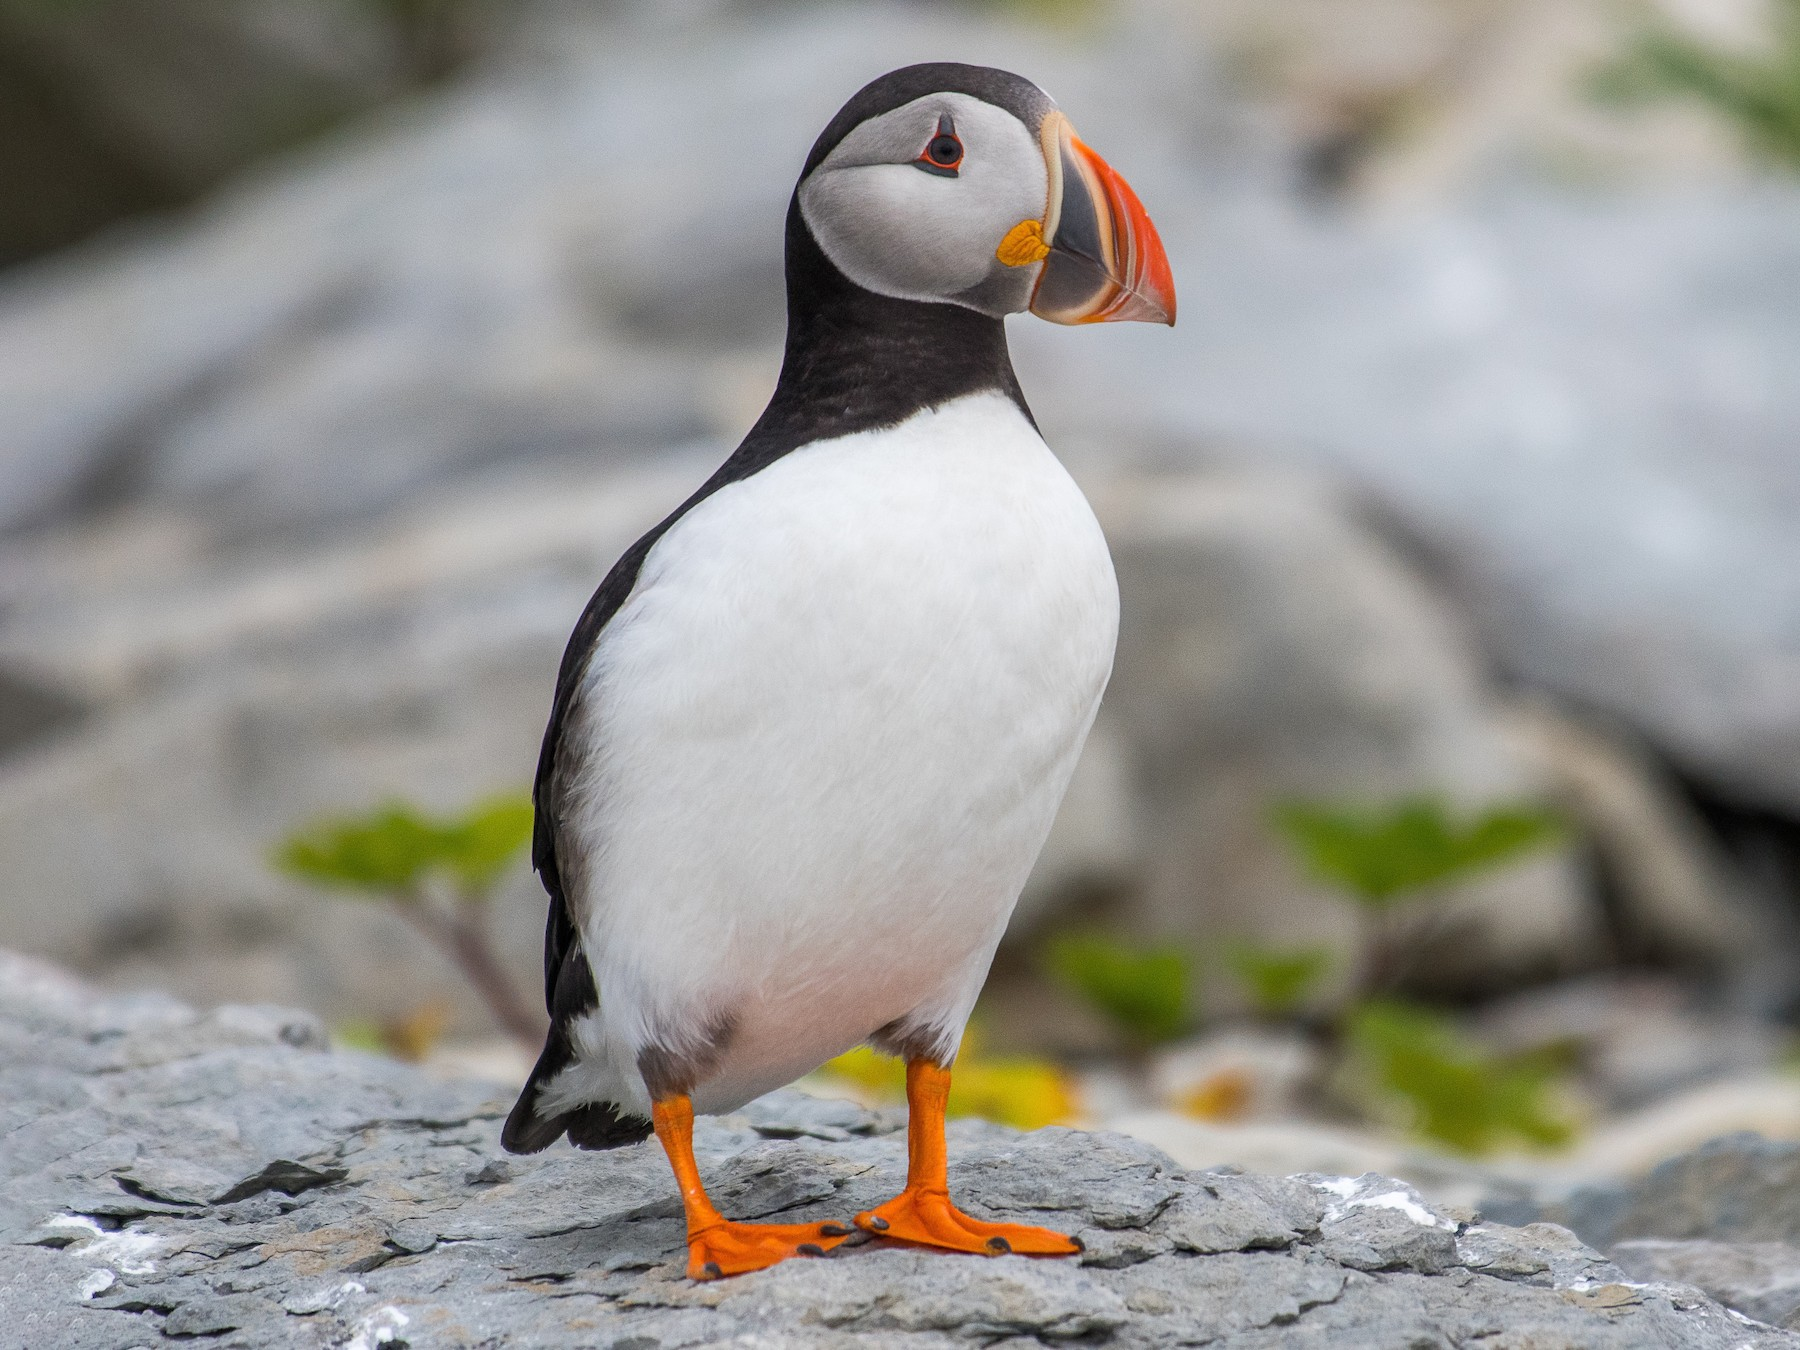
\includegraphics[width=10cm]{plots/puffin.jpeg}
%     \caption{Atlantic Puffin}
%     \label{fig:puffin}
% \end{figure}

% \begin{figure}
%     \centering
%     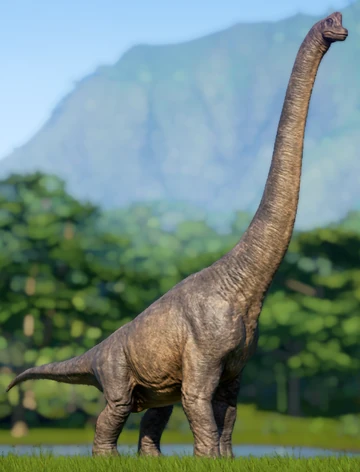
\includegraphics[width=10cm]{plots/sauropod.png}
%     \caption{Brachiosaurus}
%     \label{fig:sauropod}
% \end{figure}

% ----- Tables -----

\subsection{Tables}

% Table \ref{tab:table} shows an example of formatting a table in \LaTeX.

% \begin{table}
% 	\centering
% 	\label{tab:table}
% 	\begin{tabular}{lccr} % four columns, alignment for each
% 		\hline
% 		A & B & C & D\\
% 		\hline
% 		1 & 2 & 3 & 4\\
% 		2 & 4 & 6 & 8\\
% 		3 & 5 & 7 & 9\\
% 		\hline
% 	\end{tabular}
%     \caption{This is an example table (captions appear above tables).}
% \end{table}

% ----- Code snippets -----

\subsection{Code examples}

% You can insert snippets of code using the `tt' typewriter font:\\
% {\tt code code code}

% Or using the 'listings' package, which can format code text in a specified language:

% \begin{lstlisting}[language=Python]
% def linear(x, a, b):
%     return a*x + b
% y = linear(x, a=2, b=3)
% \end{lstlisting}

% ----- Maths -----

\subsection{Maths}

% Maths can be imbedded in the text e.g. $2^2 = 4$,  $x = a-b$, but more complicated equations should have their own space:

% \begin{equation}
%     x = \frac{-b \pm \sqrt{b^2 - 4ac}}{2a}.
% 	\label{eq:quadratic}
% \end{equation}

% Equations can be labelled and referred to in the text: the quadratic formula is defined in equation \ref{eq:quadratic}. 
% See \href{https://tug.ctan.org/info/undergradmath/undergradmath.pdf}{here} for a \LaTeX\ equation cheat sheet.

% ----- Appendices -----

% \newpage
% \appendix
% \section{Extras}

% ----- References -----

\newpage
\bibliographystyle{agsm}
\bibliography{main.bib}

\end{document}